\documentclass[border=4pt]{standalone}
\usepackage{tikz}
\usetikzlibrary{arrows.meta,calc}

\begin{document}
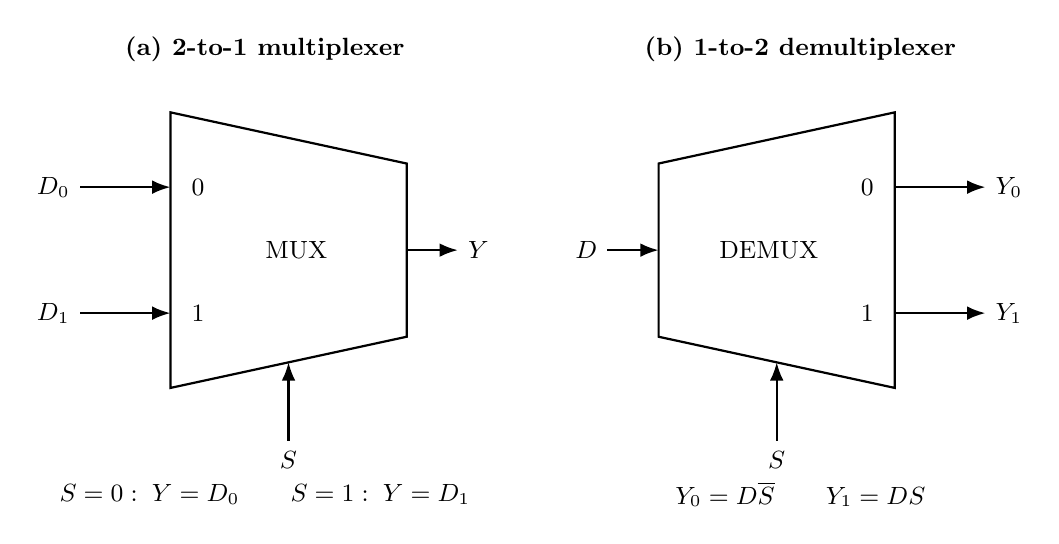
\begin{tikzpicture}[>=Latex, line width=0.8pt, font=\small]
  \node[font=\small\bfseries] at (3.2,5.1)
    {(a) 2-to-1 multiplexer};
  \draw (2.0,0.8) -- (5.0,1.45) -- (5.0,3.65) -- (2.0,4.3) -- cycle;
  \draw[<-] (2.0,3.35) -- ++(-1.15,0)
    node[left] {$D_0$};
  \draw[<-] (2.0,1.75) -- ++(-1.15,0)
    node[left] {$D_1$};
  \draw[->] (5.0,2.55) -- ++(0.65,0)
    node[right] {$Y$};
  \draw[<-] (3.5,1.125) -- ++(0,-1.0)
    node[below] {$S$};
  \node at (2.35,3.35) {0};
  \node at (2.35,1.75) {1};
  \node[align=center] at (3.6,2.55) {MUX};

  \node[font=\small\bfseries] at (10.0,5.1)
    {(b) 1-to-2 demultiplexer};
  \draw (8.2,1.45) -- (11.2,0.8) -- (11.2,4.3) -- (8.2,3.65) -- cycle;
  \draw[<-] (8.2,2.55) -- ++(-0.65,0)
    node[left] {$D$};
  \draw[->] (11.2,3.35) -- ++(1.15,0)
    node[right] {$Y_0$};
  \draw[->] (11.2,1.75) -- ++(1.15,0)
    node[right] {$Y_1$};
  \draw[<-] (9.7,1.125) -- ++(0,-1.0)
    node[below] {$S$};
  \node at (10.85,3.35) {0};
  \node at (10.85,1.75) {1};
  \node[align=center] at (9.6,2.55) {DEMUX};

  \node[align=center] at (3.2,-0.55)
    {$S=0:\;Y=D_0$\qquad $S=1:\;Y=D_1$};
  \node[align=center] at (10.0,-0.55)
    {$Y_0=D\overline S$\qquad $Y_1=DS$};
\end{tikzpicture}
\end{document}
